\section{Fremstilling og prissætning} \label{Fremstillingsmetoder}
Til fremstillingen af produktet kræves der en række forskellige fremstillingsmetoder. I følgende afsnit udvælges enkelte dele hvorefter der beskrives hvilke fremstillingsprocesser disse dele skal igennem før de kan monteres på det endelige produkt. Produktet gør brug af dele lavet ved en række metoder, bland andet ekstrudering, som beskrives i \ref{alu Ekstrudering} herunder, samt dele lavet ved spåndtagning.


\subsection{Fremstilling af monteringsblok} % Ved ikke helt hvad jeg skal kalde dette kapitel
De dele der skal laves internt kan laves ved brug af CNC fræsere og drejebænke. Disse dele vil alle blive lavet af EN-AW 6082 - T6, denne aluminiumslegering har god styrke, bearbejdelighed og pris. Nogle af delene vil være lettere at lave ved hjælp af et "rotary table", dette er en monteringsblok man sætter på fræserens bord, der tillader at rotere emnet. Dette bruges for at mindske hvor gange emnet skal afmonteres for at bearbejde det. Hver gang emnet fjernes fra indspændingen skal maskinens koordinatsystem nulstilles, hvilket gør det sværere at opnå præcision. Herunder gennemgås en mulig måde hvorpå monterings blokken kan fremstilles, det er vigtigt at pointere at dette ikke nødvendigvis er den bedste måde at fremstille delen på, da der mangler viden i projektet om fremstilling. 

\begin{figure}[H]
    \begin{subfigure}[b]{0.48\textwidth}
        \centering
        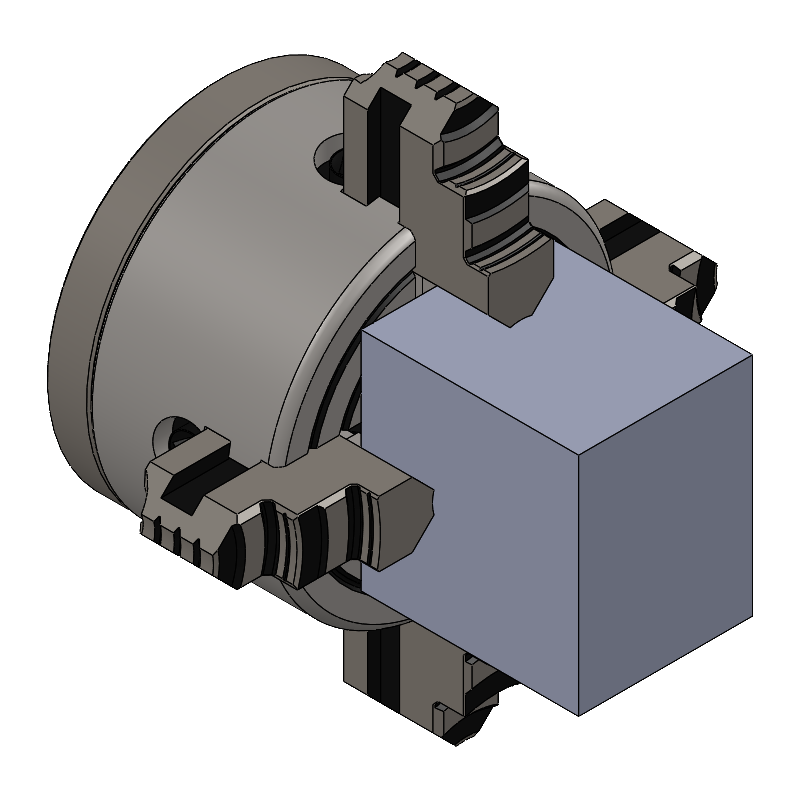
\includegraphics[width=0.8\linewidth]{Sections/6 Detaljeløsning/Media/StepByStep/Step 0.png}
        \caption{Tilskårede materiale fastspændt i chuncken, der er monteret i et rotary table.}
        \label{fig:Step0}
    \end{subfigure}
    \hfill
    \begin{subfigure}[b]{0.48\textwidth}
        \centering
        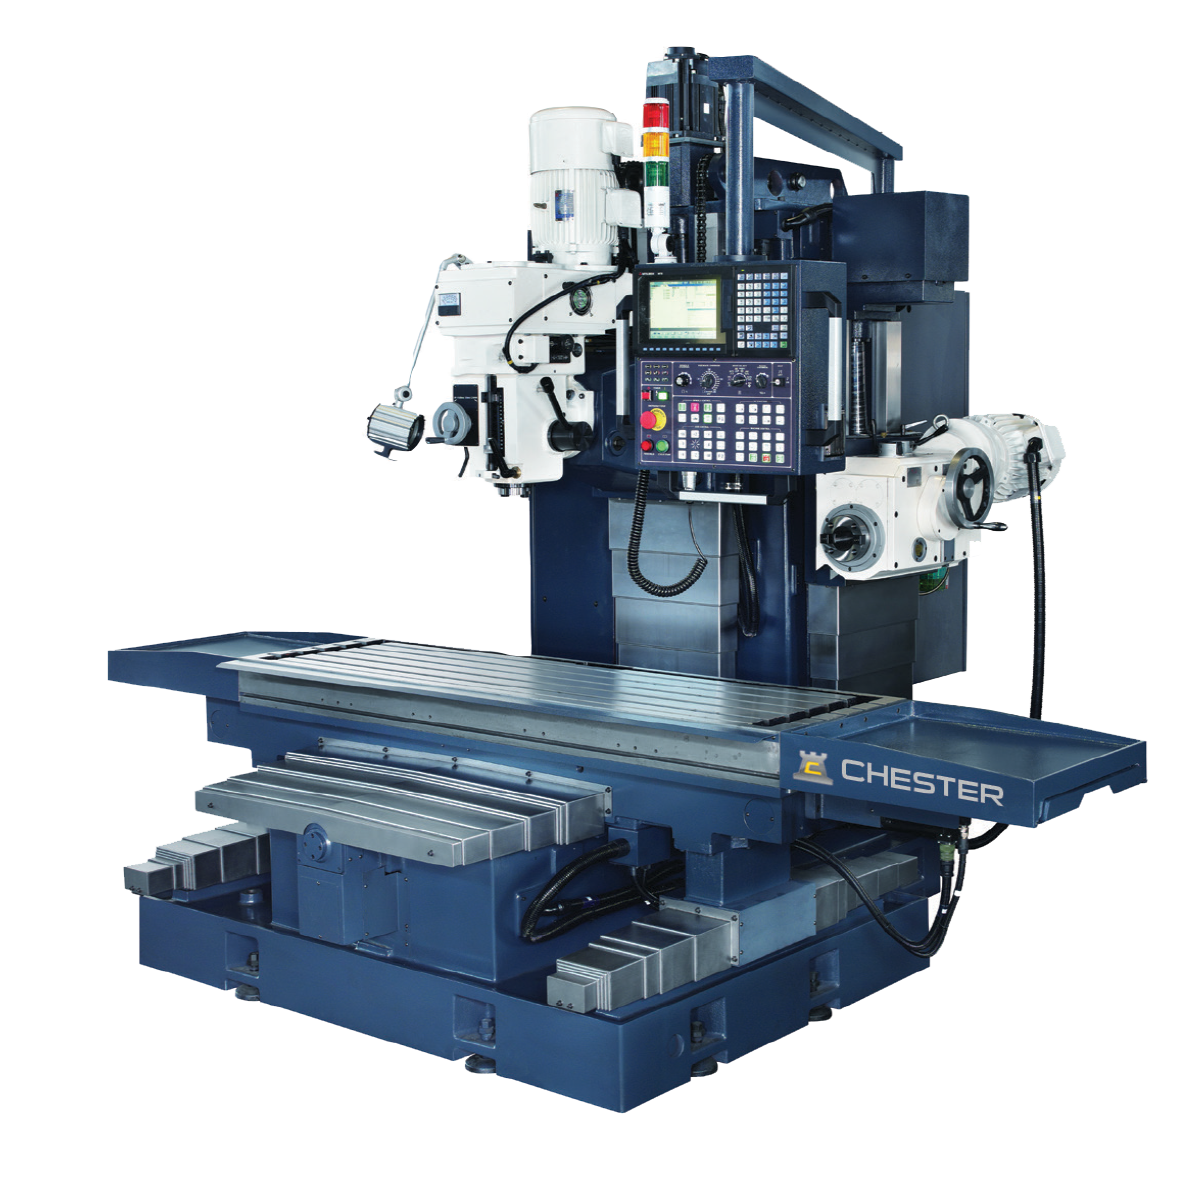
\includegraphics[width=0.8\linewidth]{Sections/6 Detaljeløsning/Media/Vertical-Horizontal-Bed-Type-CNC-Milling-Machine-•-Chester-•-GM1500VS-3222663431.png}
        \caption{Eksempel på en vertikal fræser fra \parencite{CHESTER2025GM1500VSTools}}
        \label{fig:VerticalMill}
    \end{subfigure}
    \\
    \begin{subfigure}[b]{0.48\textwidth}
        \centering
        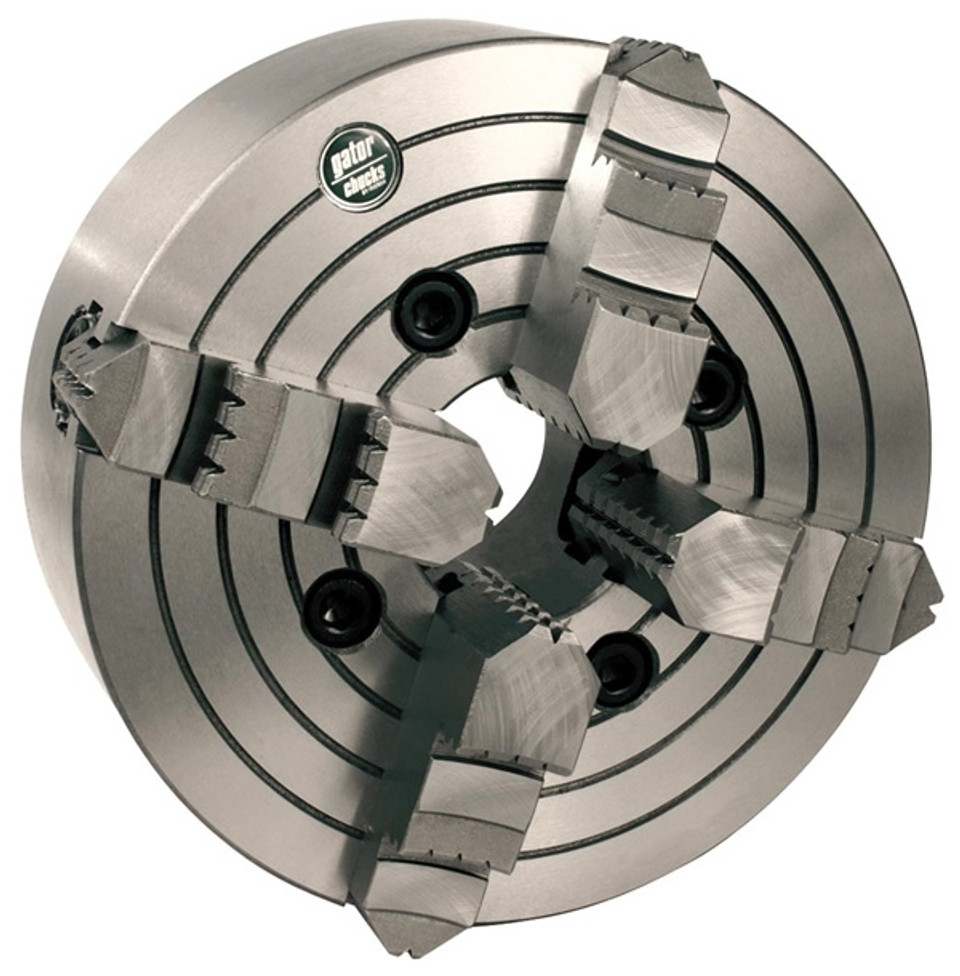
\includegraphics[width=0.8\linewidth]{Sections/6 Detaljeløsning/Media/63-718-004-gator__55302.1565719491-1329413139.jpg}
        \caption{Eksempel på en 4 Jaw chuck fra Gator \parencite{PennToolCo.2025GatorInc}}
        \label{fig:Chuck}
    \end{subfigure}
    \hfill
    \begin{subfigure}[b]{0.48\textwidth}
        \centering
        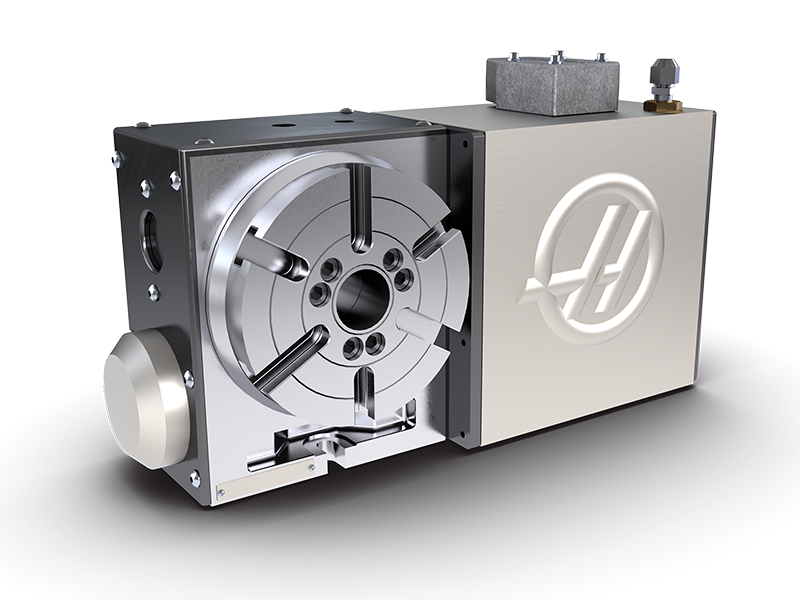
\includegraphics[width=0.9\linewidth]{Sections/6 Detaljeløsning/Media/rotarytable.png}
        \caption{Eksempel på Rotary Table fra \parencite{Haas2025RotaryTables}}
        \label{fig:RotTable}
    \end{subfigure}
\caption{Herunder ses eksempler på det nødvendige maskineri samt udgangspunkter for processen.}
\end{figure} \plainbreak{-.5}

Delen starter som en \(\SI{55}{mm}\) \(\times\) \(\SI{55}{mm}\) \(\times\) \(\SI{55}{mm}\) blok af aluminium 6082-T6 der skæres ud og planes. Man står nu med en blok der er klart til at blive behandlet. Den indspændes i en 4-jaw chuck ((\ref{fig:Chuck}) der er sat i et rotary table (\ref{fig:RotTable})). Herunder ses processen trinvis. For mange af disse trin fjernes størstedelen af materialet ved at tage grove og mindre præcise cuts, efterfulgt af finere og mere præcise cuts, der fjerner mindre materiale.



\begin{figure}[H]
    \centering
    % First row of images
  %  \begin{minipage}[t]{\textwidth}
        \begin{subfigure}[t]{0.32\textwidth}
            \centering
            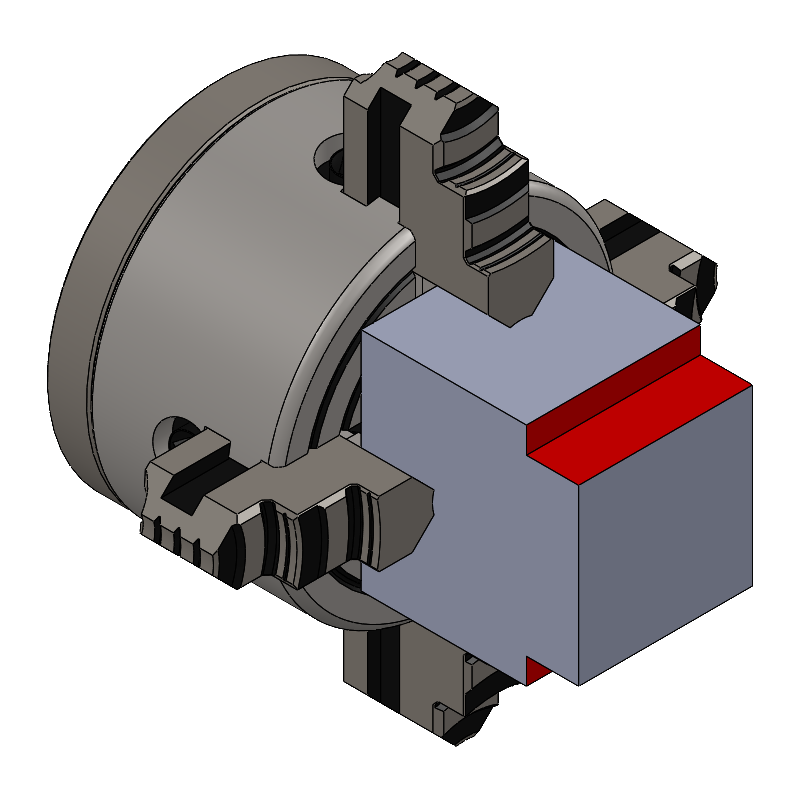
\includegraphics[width=0.9\linewidth]{Sections/6 Detaljeløsning/Media/StepByStep/Step 1.png}
            \caption{Et $\SI{6}{\milli\meter}$ dybt og $\SI{12}{\milli\meter}$ bredt område fræses væk med endefræsning; dette gøres på begge sider.}
            \label{fig:Step1}
        \end{subfigure}
        \hfill
        \begin{subfigure}[t]{0.32\textwidth}
            \centering
            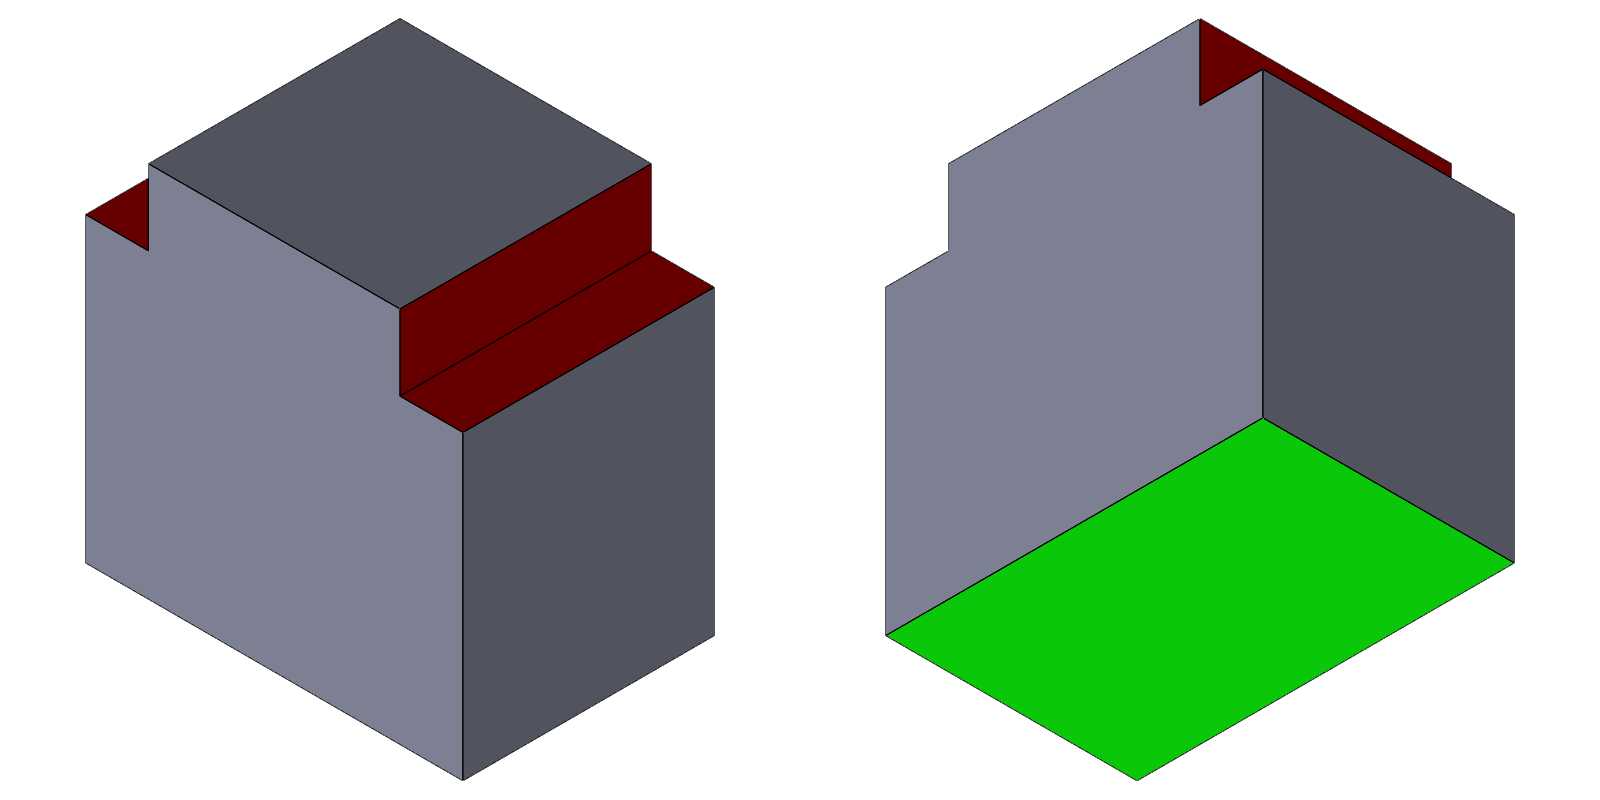
\includegraphics[width=0.9\linewidth]{Sections/6 Detaljeløsning/Media/StepByStep/Step 2.png}
            \caption{Med et fasværktøj fræses en $\SI{6}{\mm} \times \SI{45}{\degree}$ fas som vist ovenfor, dette udføres på begge sider.}
            \label{fig:Step2}
        \end{subfigure}
        \hfill
        \begin{subfigure}[t]{0.33\textwidth}
            \centering
            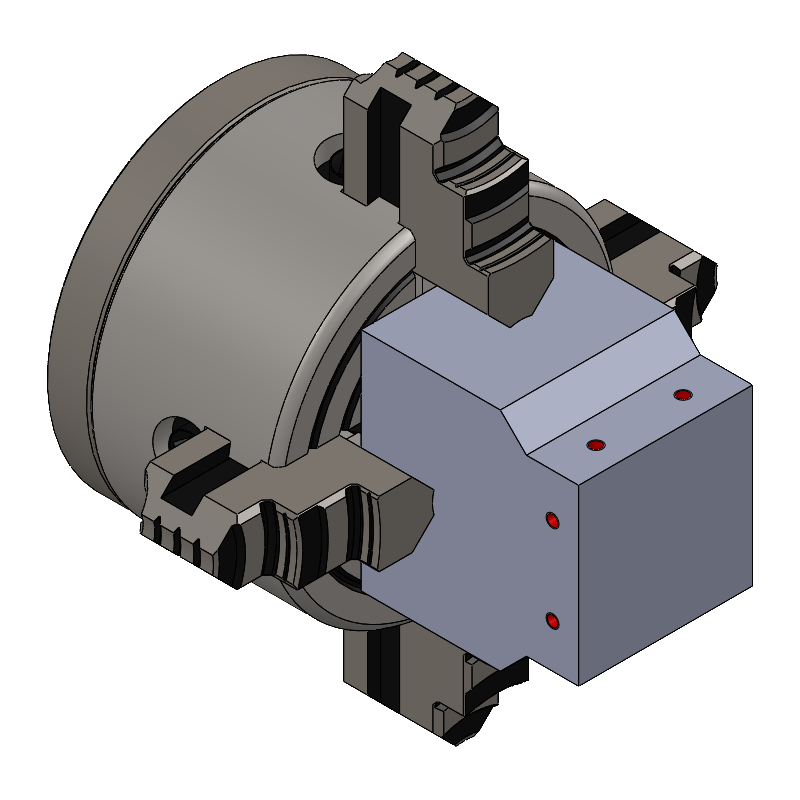
\includegraphics[width=0.9\linewidth]{Sections/6 Detaljeløsning/Media/StepByStep/Step 3.png}
            \caption{Gevindhuller fremstilles ved først at bore et hul, i dette tilfælde med et $\SI{2.5}{\milli\meter}$ bor, hvorefter der anvendes en gevindtap. Denne proces gentages på alle fire sider.}
            \label{fig:Step3}
        \end{subfigure}
   % \end{minipage}
    
    \vspace{1em}
    %\begin{center}
      %  \small Emnet fjernes og vendes for at blive fastspændt ved den netop bearbejdede flade
   % \end{center}
  %  \vspace{1em}
    
    % Second row of images
  %  \begin{minipage}[t]{\textwidth}
        \begin{subfigure}[t]{0.32\textwidth}
            \centering
            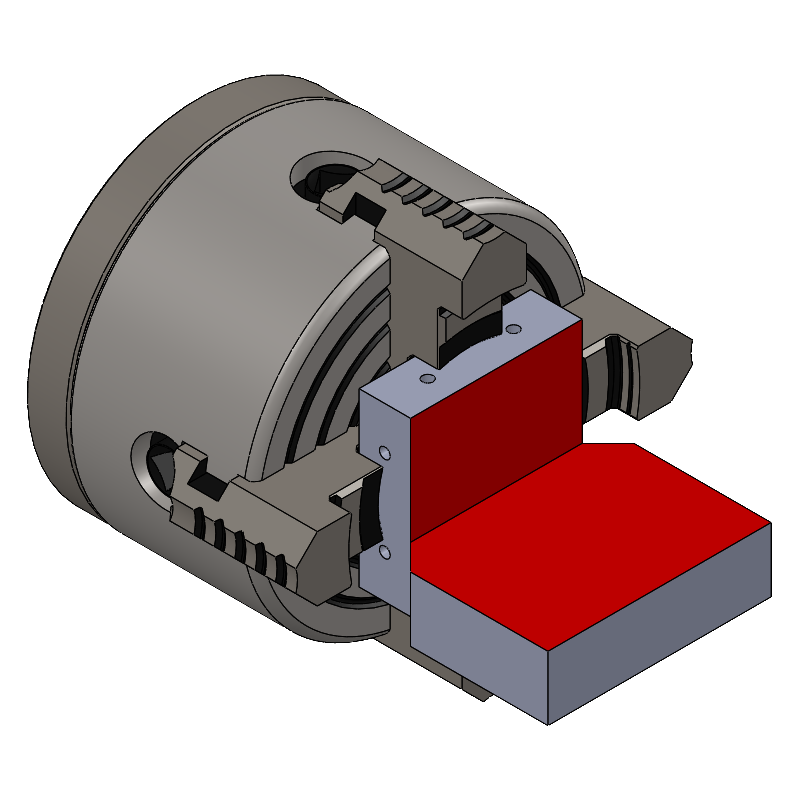
\includegraphics[width=0.9\linewidth]{Sections/6 Detaljeløsning/Media/StepByStep/Step 4.png}
            \caption{Dette er et omfattende trin, som kræver mange snit med en endefræser. Dette kræver opmærksomhed for at undgå at deformere emnet, da en stor mængde materiale skal fjernes}
            \label{fig:Step4}
        \end{subfigure}
        \hfill
        \begin{subfigure}[t]{0.32\textwidth}
            \centering
            \includegraphics[width=0.9\linewidth]{Sections/6 Detaljeløsning/Media/StepByStep/Step 5.png}
            \caption{Emnet roteres, og igen anvendes et fasværktøj, dimensionerne er de samme som i trin 2.}
            \label{fig:Step5}
        \end{subfigure}
        \hfill
        \begin{subfigure}[t]{0.32\textwidth}
            \centering
            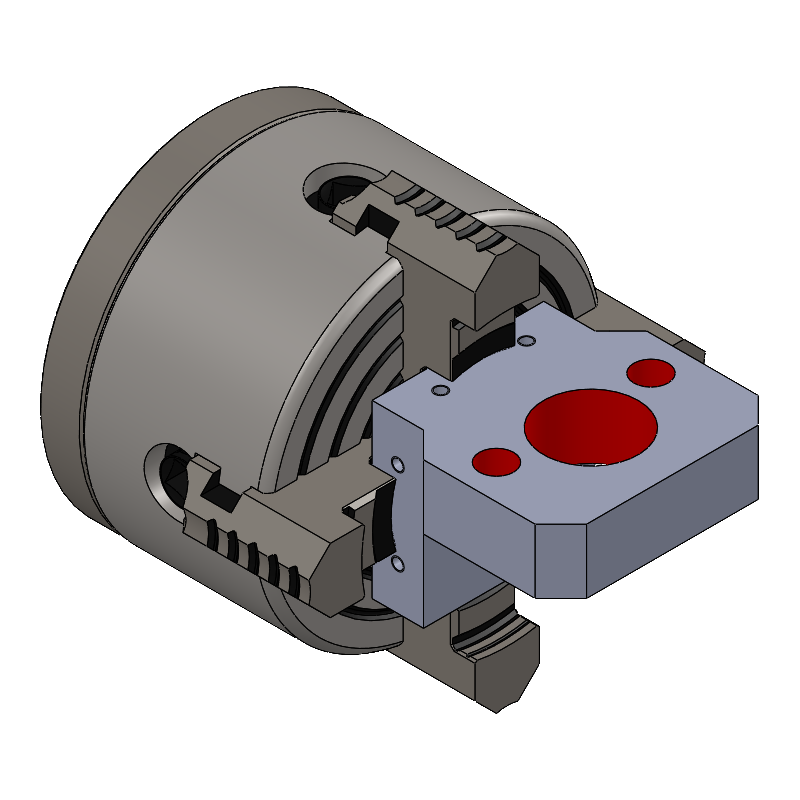
\includegraphics[width=0.9\linewidth]{Sections/6 Detaljeløsning/Media/StepByStep/Step 6.png}
            \caption{Det centrale hul kan bores i ét trin hvis et \SI{22}{mm} bor ejes, ellers må det fræses ud. De to mindre huller kræver en plan bund, så værktøjs udvalget bestemmer processen. Selvom fladbundsbor findes, kan hullerne også fræses.}
            \label{fig:Step6}
        \end{subfigure}
   % \end{minipage}
    
    \vspace{1em}
    
    % Third row of images
    %\begin{minipage}[t]{\textwidth}
        \begin{subfigure}[t]{0.32\textwidth}
            \centering
            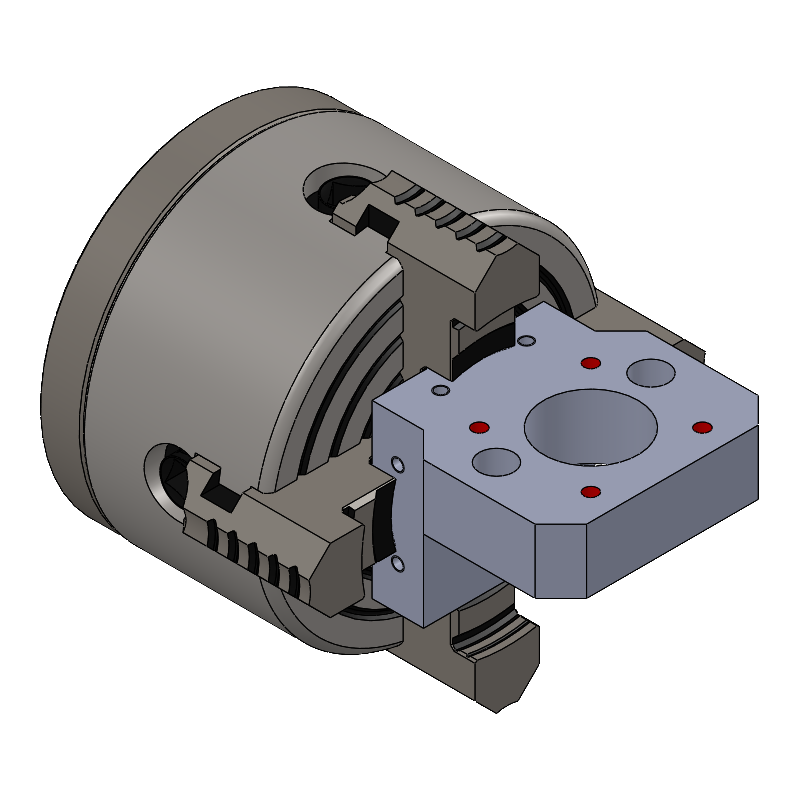
\includegraphics[width=0.9\linewidth]{Sections/6 Detaljeløsning/Media/StepByStep/Step 7.png}
            \caption{I modsætning til de tidligere huller er disse ikke med gevind, men de er forsænkede. Først bores et frigangshul til M3 med en diameter på $\SI{3.4}{\milli\meter}$. Da det er gennemgående huller kan de bare bores.}
            \label{fig:Step7}
        \end{subfigure}
        \hfill
        \begin{subfigure}[t]{0.32\textwidth}
            \centering
            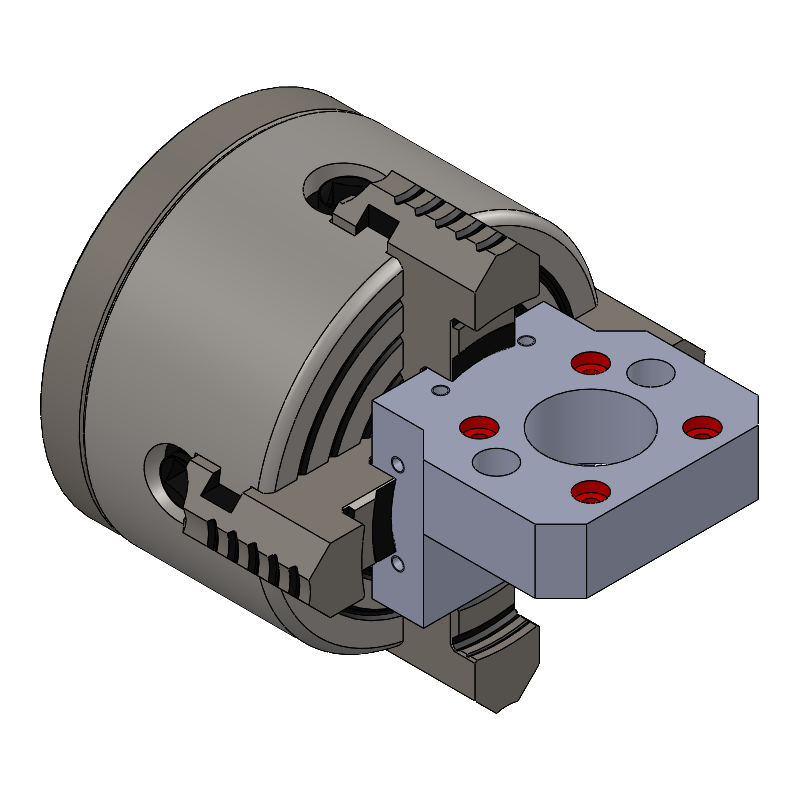
\includegraphics[width=0.9\linewidth]{Sections/6 Detaljeløsning/Media/StepByStep/Step 8.png}
            \caption{Næste trin er forsænkningerne. For de anvendte bolte er en forsænkning på $\SI{6.40}{\milli\meter}$ i diameter og $\SI{2.4}{\milli\meter}$ i dybde nødvendig. Dette kan udføres med en forsænker, som centreres i de tidligere borede huller.}
            \label{fig:Step8}
        \end{subfigure}
        \hfill
        \begin{subfigure}[t]{0.32\textwidth}
            \centering
            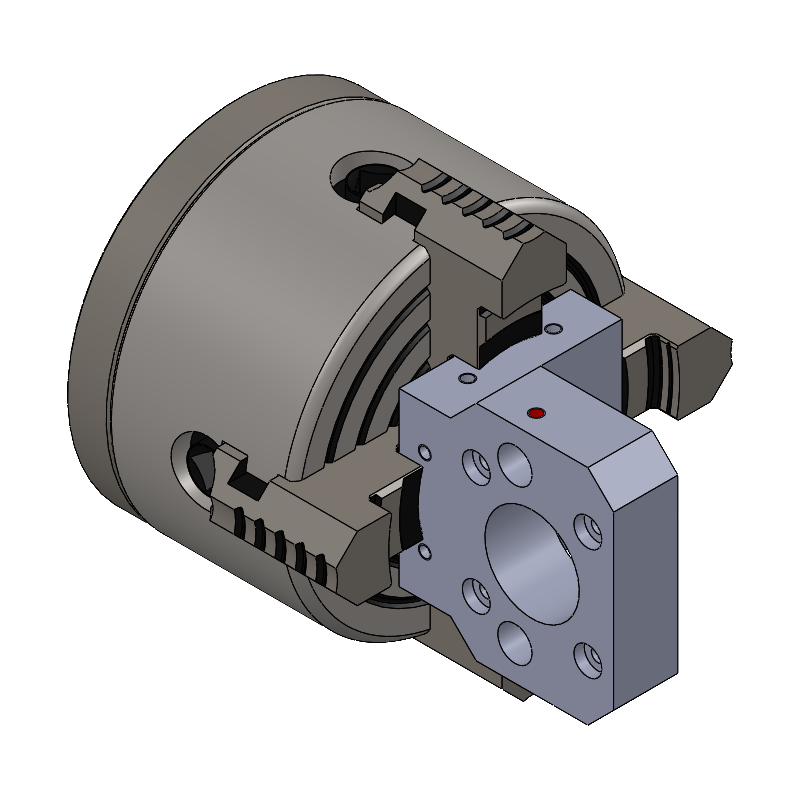
\includegraphics[width=0.9\linewidth]{Sections/6 Detaljeløsning/Media/StepByStep/Step 9.png}
            \caption{Det sidste trin er hul og gevind til M4-pinol skruerne der fastgør akslerne. Processen er den samme som i trin 3, blot med en M4-gevindtap og et $\SI{3.25}{\milli\meter}$ bor.}
            \label{fig:Step9}
        \end{subfigure}
   % \end{minipage}
    
    \caption{Trin-for-trin fremstillingsproces af emnet. Emnet fjernes og vendes mellem \textit{(c)} og \textit{(d)}, for at blive fastspændt ved den netop bearbejdede flade}
    \label{fig:stepbystep}
\end{figure}


%Gevindholderen til indspændingssystemet (se figur \ref{fig:Gevindholder-frem}) er fremstillet af en rustfri stålstang og udgør det faste element, som M6-boltene skrues ind i, når emnet skal fastholdes på bundpladen. Gevindholderen er dreget i ét stykke rustfrit stål, så dens ydre cylindriske form med diameter på 16 mm let kan vinkles mod emnet og fordele spændekraften jævnt, også på skrå overflader. 
%Under fremstilling skæres en Ø16 stang til, hvorefter den på en CNC-drejebænk bearbejdes med en indsnævring på 10 mm i den ene ende, så den passer i de tilsvarende huller på arbejdspladen. I en CNC-fræser  bearbejdes den med to gennemgående M6-gevind, med en frihøjde på henholdsvis 3 og 16 mm indsnævringen og derved arbejdspladen. Efter gevindskæring slibes og affases enderne for at fjerne grader, og hele holderen poleres for at beskytte gevindets tolerance ($\pm$ 0,1 mm) og sikre problemfri boltføring. 



%\begin{figure}[H]
%    \centering
%    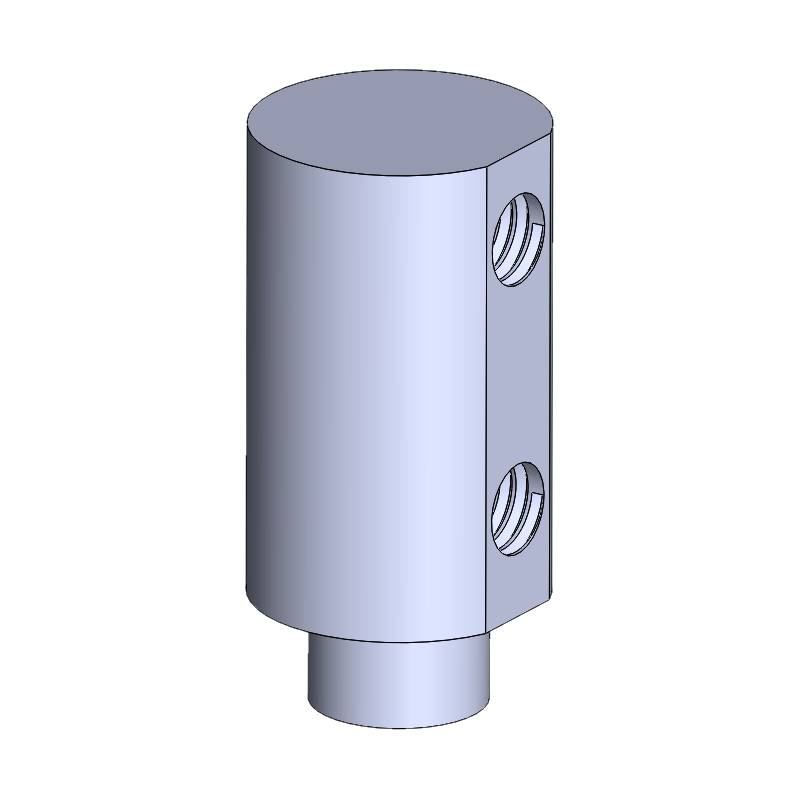
\includegraphics[width=0.5\linewidth]{Sections/6 Detaljeløsning/Media/Billeder til indspænding/Gevindholder.png}
%    \caption{Gevindholder}
%    \label{fig:Gevindholder-frem}
%\end{figure}

\subsection{Aluminiums profiler} \label{alu Ekstrudering} \plainbreak{-.5}
Til konstruktion af robottens stativ er der anvendt T-slotprofiler i aluminium (se figur \ref{fig:T-slot profil}), som er fremstillet ved ekstrudering. Ekstrudering er en kontinuerlig produktionsproces, hvor et opvarmet aluminiumsemne kaldet en billet - presses gennem en form (matrice) der er profilens ønskede tværsnit. Ved hjælp af højt tryk og temparatur opnås en ensartet, langstrakt profil med præcis geometri.\parencite{Johnson1962TheExtrusion} 

Processen begynder med forvarmning af aluminiumsbilletten til cirka 450-500 grader °C, hvorefter den presses gennem matricen med en hydraulisk presse. Når profilen forlader matricen, afkøles den kontrolleret med luft eller vand for at opretholde den dimensionelle stabilitet. Efter afkøling rettes profilen mekanisk, og overskydende materiale i enderne fjernes. Til sidst varmebehandles profilerne (typisk T5 eller T6-hærdning) for at opnå den ønskede styrke og hårdhed. Til applikationen i projektet tages disse lange profiler og tilskæres de ønskede længder der skal bruges. \parencite{Johnson1962TheExtrusion} 
 
\begin{figure}[H]
    \centering
    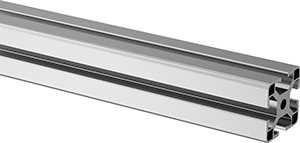
\includegraphics[width=0.35\linewidth]{Sections/6 Detaljeløsning/Media/T-slots.png}
    \caption{T-slot alu profilrør. \parencite{McMaster-Carr2025T-SlottedRails}}
    \label{fig:T-slot profil}
\end{figure} \plainbreak{-.5}


\plainbreak{0.2}
\subsection{Samling} \label{samling}
Ekstrudering er en økonomisk og præcis fremstillingsmetode, der muliggør høj gentagelsesnøjagtighed og lav materialespild \parencite{Johnson1962TheExtrusion}. Desuden er aluminium velegnet til robotstativet grundet dets lave vægt og tilstrækkelige mekaniske styrke, se afsnit. 

Ses der på den samlede konstruktion af robotten er den primære samlingsmetode bolte. Hele robotstrukturen er opbygget som en modulær skruesamling, hvor alle mekaniske komponenter, fra T-slot-rammen over følgestænger og motorbeslag til doseringshoved, fastgøres med standard skruer. På aluminiumsprofilerne anvendes T-slot-notsten, som glider ind i profilens riller, hvorefter en skrue bruges til at montere beslag, motorer og så videre. Hvordan dette samles kan ses i bilag \ref{Bilag - arbejdstegniner}.

\begin{table}[H]
\setlength{\tabcolsep}{20pt}
 \centering
  \caption{Værktøjsliste}
 \begin{tabular}{|l l|} \hline
  \multicolumn{2}{|c|}{\cellcolor{aaublue} \color{white} \textbf{Værktøjsliste}}  \\\hline
 \rowcolor{gray!10} \multicolumn{1}{|c}{\textbf{Navn}} &  \multicolumn{1}{c|}{\textbf{Anvendelsessted}}  \\\hline

  10 mm fastnøgle & Indspænding  \\\hline
  4 mm umbracho nøgle & \makecell{Indspænding \\ Samling af stellet \\ Lineær bevægelse}  \\\hline
  2 mm umbracho nøgle & \makecell{Lineær bevægelse }  \\\hline
 
 \end{tabular}
 \label{tab: værktøjsliste}
\end{table}

Til samling af speckle pattern robotten benyttes tre standard værktøj, som fremgår af tabel \ref{tab: værktøjsliste}.





